%!TEX TS-program = xelatex
%!TEX encoding = UTF-8 Unicode

\documentclass[11pt,tikz,border=1]{standalone}
\usepackage{pgfplots}
\usetikzlibrary{positioning}

\begin{document}
  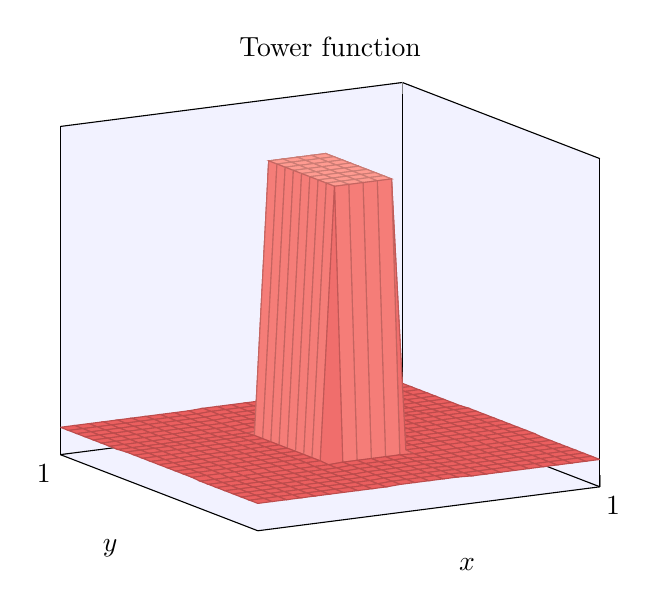
\begin{tikzpicture}
  
      \begin{axis}[
        view={-30}{15},        
        axis background/.style={fill=blue!5},
        xlabel=$x$,
        ylabel=$y$,
        xtick distance=1,
        ytick distance=1,
        ztick distance=1,
        xtick={1},
        ytick={1},
        ztick={2},  % big number to disable
        title={Tower function},
        colormap={simple}{rgb255=(235,95,95) rgb255=(255,155,145)},
        declare function={
          sigma(\z)=1/(1 + exp(-\z));
 		  f(\x,\y,\h,\b)=sigma(\b + \h * (sigma(1000 * (\x - 0.4)) - sigma(1000 * (\x - 0.6)))	+ \h * (sigma(1000 * (\y - 0.3)) - sigma(1000 * (\y - 0.7))));
 		% f(x,y,h,b) is used in tower_construction.tex
       }]
        \addplot3[surf,domain=0:1] {
        	f(x,y,10,-16)
        };
      \end{axis}
    
  \end{tikzpicture} 
\end{document}
